\chapter{Ricorsione ed iterazione}\label{cap:ricorsione}
\section{La ricorsione}
In informatica il concetto di ricorsione è estremamente importante in quanto permette di ottenere spesso una descrizione chiara e concisa degli algoritmi. Diciamo che un algoritmo è \textit{ricorsivo} se figurano in esso delle procedure ricorsive, ovvero procedure che invocano, direttamente o indirettamente, sé stesse. Come abbiamo visto fino a questo momento, questa tipologia di algoritmi costituiscono il metodo più naturale di risoluzione di un problema in quanto sono facili da comprendere e analizzare. Infatti:
\begin{itemize}
	\item La correttezza di un programma ricorsivo si dimostra facilmente utilizzando il \textit{principio di induzione};
	\item Il calcolo della complessità temporale di un algoritmo ricorsivo si riduce alla soluzione delle equazioni di ricorrenza (come si vedrà nel Capitolo \ref{cap:ricorrenze}).
\end{itemize}
Affinché un algoritmo ricorsivo non continui a girare all'infinito deve avere le seguenti proprietà:
\begin{enumerate}
	\item Devono esistere dei criteri, detti \textbf{criteri di base} (o anche \textit{casi base}), per i quali la procedura non richiami sé stessa;
	\item Ogni volta che la procedura chiama sé stessa, essa deve essere più vicina ai criteri di base.
\end{enumerate}
Una procedura ricorsiva dotata di queste due proprietà si dice \textbf{ben definita}.

Il prodotto dei numeri interi positivi da $1$ a $n$ compresi prende il nome di ``fattoriale di $n$'' e si indica con il simbolo $n!$:
\begin{equation}
	n! = 1 \cdot 2 \cdot 3 \cdot \cdots (n-2) \cdot (n-1) \cdot n
\end{equation}
Per definizione si pone $0!=1$ quindi è possibile definire una funzione ben definita per tutti i numeri naturali. Si dimostra per induzione che:
\begin{equation}
	n! = \begin{cases}
		1 & \text{se } n=0\\
		n \cdot(n-1)!& \text{se } n>0
	\end{cases}
\end{equation}
Questa definizione di $n!$ è ricorsiva, infatti quando si usa $(n-1)!$ si sta eseguendo una ``chiamata'' alla funzione stessa. Questa definizione è ben definita in quanto il valore $n!$ è esplicitamente assegnato quando $n=0$ ed inoltre il valore $n!$ è definito in funzione di un valore più piccolo di $n$, più vicino quindi al valore di base $0$. Per calcolare, ad esempio, $4!$ saranno necessari nove passaggi. Infatti:
\begin{enumerate}
	\item $4!=4 \cdot 3!$
	\item \hspace{1cm} $3!=3 \cdot 2!$
	\item \hspace{2cm} $2!=2 \cdot 1!$
	\item \hspace{3cm} $1!=1 \cdot 0!$
	\item \hspace{4.5cm} $0!=1$
	\item \hspace{3cm} $1!=1 \cdot 1 = 1$
	\item \hspace{2cm} $2!=2 \cdot 1 = 2$
	\item \hspace{1cm} $3!=3 \cdot 2 = 6$
	\item $4!=4 \cdot 6 = 24$
\end{enumerate}


Vediamo ora una procedura che calcola il fattoriale:
	\begin{lstlisting}[language=asd,caption={\textsc{factorial\_rec}(N)},label=lst:factR]
		if N = 0 then
			fact = 1
		else
			x = factorial_rec(n-1)
			fact = N * x
		return fact;
	\end{lstlisting}

Non tutti i linguaggi di programmazione, però, supportano la ricorsione\footnote{Pascal e Cobol ad esempio non la permettono.}. La ricorsione, infatti, non è un meccanismo proprio del calcolatore il quale, come si è detto quando si è parlato di macchine astratte (vedi Sezione \ref{sez:Turing}), ha un insieme limitato di operazioni ed opera mediante assegnazioni e salti\footnote{Infatti in un calcolatore non è neanche definito il concetto di ciclo ed iterazione.}.

I linguaggi che permettono la ricorsione utilizzano in fase di esecuzione uno \textbf{stack} per tenere traccia della sequenza di chiamata delle varie procedure ricorsive. In testa a tale stack è sempre presente il \textit{record di attivazione} contenente il \textbf{contesto} della procedura correntemente attiva. Tale contesto comprende:
\begin{itemize}
	\item le variabili locali alla procedura;
	\item i parametri ad essa passati;
	\item l'indirizzo di ritorno, ovvero il contenuto del \textit{program counter} nel momento in cui la procedura è stata invocata.
\end{itemize}

Quando una procedura è invocata viene posto sulla pila un nuovo record di attivazione. Ciò indipendentemente dal fatto che siano già presenti nella pila altri record di attivazione relativi alla stessa procedura. Per questo motivo la ricorsione è molto dispendiosa in termini di memoria. Più in avanti vedremo alcuni esempi di algoritmi ricorsivi che non richiedono l'utilizzo di uno stack.

\section{La traduzione da ricorsivo ad iterativo}
\subsection{La memoria di lavoro}
Come abbiamo visto, la ricorsione è un meccanismo che non è proprio del calcolatore. Per questo motivo, quando si scrive un programma ricorsivo, il compilatore deve tradurlo in un programma iterativo. Alla base di questa traduzione c'è il concetto di \textbf{memoria di lavoro} che è una memoria ausiliaria che viene utilizzata per salvare i dati necessari al calcolo di una procedura ricorsiva. In particolare, la memoria di lavoro è costituita da uno \textbf{stack} che viene utilizzato per salvare i \textbf{parametri formali} delle varie chiamate ricorsive. Ogni volta che è necessario eseguire una sottochiamata ricorsiva ci si avvale della memoria di lavoro per salvare i parametri formali della procedura corrente per poterli poi recuperare al ritorno dalla chiamata ricorsiva. In questo modo, la memoria di lavoro permette di simulare la ricorsione mediante iterazione.

\subsection{Uno schema generale per la traduzione}
\subsubsection{Il ciclo while}
La traduzione di un algoritmo ricorsivo in un algoritmo iterativo richiede un approccio basato su un grande ciclo \texttt{while} il quale gestisce al suo interno le due fasi principali di una chiamata ricorsiva: l'\textbf{inizializzazione} di una nuova chiamata ricorsiva e il \textbf{ripristino} dei dati precedentemente utilizzati al \textit{ritorno} di una queste ultime.  Per capire quale fase bisogna gestire ci avvaliamo di una variabile booleana \texttt{start}\footnote{Negli esempi presenti nel capitolo capiterà di sostituire tale variabile con una vera e propria condizione sui parametri attuali.} che assume valore \texttt{true} quando siamo nella fase di \textit{inizializzazione} di una nuova chiamata ricorsiva e \texttt{false} quando siamo nella fase di \textit{ripresa} di una chiamata sospesa.

Oltre alla condizione sulla variabile \texttt{start}, è necessario controllare anche lo \textbf{stato dello stack}. Infatti, se lo stack è vuoto significa che \textit{non ci sono chiamate ricorsive sospese} e quindi non è necessario effettuare alcuna ripresa e si può procedere fino alla fine dell'algoritmo. In caso contrario sarà necessario \textit{ripristinare il contesto della chiamata ricorsiva sospesa} per eseguire le varie sottochiamate e proseguire con l'esecuzione dell'algoritmo.

\subsubsection{Il punto di ritorno: la variabile last}
Al ritorno da una chiamata ricorsiva bisogna cercare di capire il punto dal quale riprendere l'esecuzione della chiamata precedentemente sospesa. Per fare ciò è necessario individuare il cosiddetto \textbf{punto di ritorno}, ovvero l'istruzione che segue immediatamente la chiamata ricorsiva appena terminata. In generale, un modo per discriminare il punto di ritorno a fronte di più chiamate ricorsive è quello di utilizzare una variabile \texttt{last} la quale, \textit{ogni volta che si termina una chiamata ricorsiva}, viene aggiornata con il valore del parametro attuale che sarà sicuramente diverso dai corrispettivi delle altre sottochiamate ricorsive (in caso contrario, infatti, si avrebbero chiamate ridondanti e si finirebbe in un loop).

È possibile quindi delineare uno schema generale per la traduzione di un algoritmo ricorsivo in uno puramente iterativo come mostrato in Figura \ref{fig:schema}.

\begin{center}
	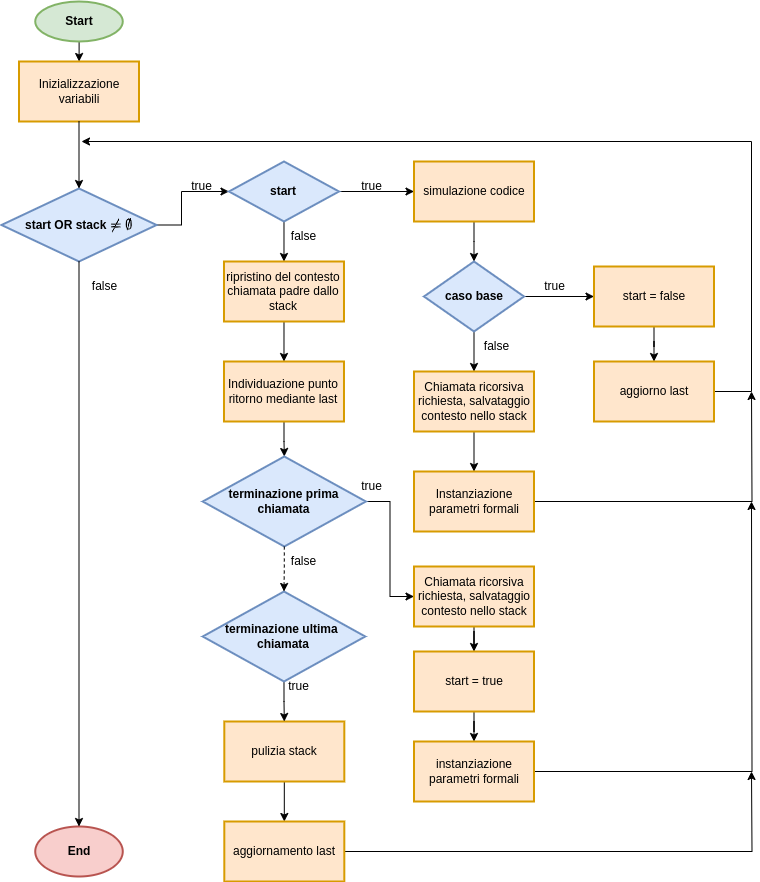
\includegraphics[scale=.6]{res/schema_traduzione}
	\captionof{figure}{Schema algoritmo iterativo che simula algoritmo ricorsivo}\label{fig:schema}
\end{center}


\subsection{La funzione fattoriale}
Osservando l'algoritmo \ref{lst:factR} notiamo che si effettuano nuove chiamate ricorsive ogni qualvolta la variabile \texttt{N} è maggiore o uguale a zero. Per questo motivo possiamo pensare di porre come condizione di loop nel ciclo \texttt{while} il controllo \texttt{cn $\geq$ n}.

Per poter ripristinare il contesto della chiamata padre, è necessario salvare in memoria i parametri formali della procedura ricorsiva. Nel caso della funzione fattoriale, per simulare l'inizio di una chiamata ricorsiva, è necessario verificare se il parametro \texttt{N} è uguale a \texttt{0} e, in caso affermativo, assegnare il valore \texttt{1} alla variabile \texttt{ret}.

Nel caso in cui \texttt{N} sia diverso da \texttt{0} è necessario eseguire una nuova chiamata ricorsiva. Per permetterlo è necessario innanzitutto salvare nello stack il valore corrente  di \texttt{N} e assegnare a \texttt{cn} (\textit{current n}) il valore \texttt{N-1} (\textbf{instanziazione parametri formali}). Sarà quindi necessario un unico stack per salvare il valore di \texttt{N}. Non è necessario salvare il valore di \texttt{fact} in quanto questo viene calcolato al ritorno dalla chiamata ricorsiva.

Chiaramente, una volta arrivati al caso base il valore \texttt{cn} sarà uguale a \texttt{-1} ma lo stack non sarà vuoto e sarà necessario effettuare nuove iterazioni per svuotarlo per ottenere il valore finale. Si ha così un primo esempio di traduzione di un algoritmo ricorsivo in un algoritmo iterativo:

\begin{lstlisting}[caption={Traduzione iterativa della funzione fattoriale},language=asd]
cn = n
stack = NIL
while (cn >= 0 || stack != NIL) do
	if cn >= 0 then
		// caso base
		if cn = 0 then
			r = 1
			ret = r
			cn = -1
		// avvio sottochiamata
		else
			// salvataggio contesto
			stack = push(stack, cn)
			// aggiorno il parametro per la sottochiamata
			cn = cn - 1
	// ritorno da sottochiamata
	else
		// ripristino contesto
		cn = top(stack)
		x = ret
		r = cn * x
		stack = pop(stack)
		ret = r
		cn = -1
return ret
\end{lstlisting}

\subsection{L'esempio del MergeSort}
Consideriamo l'algoritmo di ordinamento \texttt{Merge Sort}. Questo è un algoritmo di ordinamento ricorsivo basato sul concetto del ``divide et impera''. La sua idea principale consiste nel dividere un array non ordinato in due metà, ordinare ciascuna metà separatamente, e infine combinare le due metà ordinate in un unico array ordinato. L'algoritmo opera ricorsivamente fino a quando l'array non può essere più diviso, e poi procede a combinare le parti ordinate.

\begin{lstlisting}[caption={\textsc{MergeSort}(A,p,r)},language=asd,label={lst:mergeSortR}]
if p<r then
	q = (p+r)/2
	MergeSort(A,p,q)
	MergeSort(A,q+1,r)
	Merge(A,p,q,r)
\end{lstlisting}

Notiamo fin da subito che l'algoritmo \texttt{MergeSort} richiama se stesso due volte. Quando un compilatore traduce un programma scritto in un linguaggio di alto livello in un linguaggio di basso livello, come il linguaggio macchina, non può utilizzare la ricorsione in quanto non esiste in esso. Il compilatore deve quindi tradurre la ricorsione in iterazione.

Nell'algoritmo \ref{lst:mergeSortR} compaiono quattro variabili: \texttt{p, r, q, A}. Durante la fase di traduzione in iterazione, notiamo però che solo le variabili \texttt{p}, \texttt{q} ed \texttt{r} vengono modificate. La variabile \texttt{A} rappresenta un puntatore alla prima cella dell'array da ordinare e che quindi non cambia mai mentre la variabile \texttt{q} viene calcolata in ogni sottochiamata dati i valori correnti di \texttt{p} ed \texttt{r} (salvati nelle variabili \texttt{cp} e \texttt{cr}), per questo motivo non sarebbe necessario memorizzare la variabile \texttt{q} ma ciò nonostante utilizzeremo tre stack, uno per ogni variabile \texttt{p, q, r}.

Per discriminare il punto di ritorno, avendo a che fare con due chiamate ricorsive, utilizzeremo la variabile \texttt{last} che verrà aggiornata ogni volta che si termina una chiamata ricorsiva. Infatti, ciascuna sottochiamata assume parametri formali diversi e ogni volta che termina deve comunicare al padre il valore del suo terzo parametro per poter proseguire con l'esecuzione. Per questo motivo, la variabile \texttt{last} conterrà il valore della variabile \texttt{cr}. Al ritorno da ciascuna sottochiamata, basterà quindi controllare se il valore di \texttt{last} è uguale al valore di \texttt{cr} per capire se si è terminata la prima o la seconda sottochiamata. Se, al termine di una iterazione, \texttt{last} è uguale a \texttt{q} allora sicuramente si sta tornando dalla terminazione della prima chiamata ricorsiva. Se invece \texttt{last} è uguale a \texttt{cr} allora non sarà necessario effettuare nuove chiamate ricorsive e si può procedere fino alla fine dell'algoritmo.

\begin{lstlisting}[caption={\textsc{MergeSort\_Iter}(A,p,r)},language=asd,label={lst:mergeSortI}]
cp = p
cr = r
stackR = NIL
stackP = NIL
stackQ = NIL
start = true
while (start || stackR != NIL) do
	if start then
		if cp < cr then
			// simulazione codice fino alla prima chiamata ricorsiva
			q = (cp+cr)/2
			// avvio prima sottochiamata, salvataggio contesto
			stackR = push(stackR, cr)
			stackP = push(stackP, cp)
			stackQ = push(stackQ, q)
			// aggiornamento parametri formali
			cr = q
		// simulazione terminazione, la chiamata padre potrebbe essere stata sospesa
		else
			last = cr
			start = false
	else
		// ripristino contesto
		cr = top(stackR)
		cp = top(stackP)
		q = top(stackQ)
		// individuazione punto di ritorno
		if last @$\neq$@ cr then
			cp = q + 1
			start = true
		else
		// fine della seconda sottochiamata, terminazione chiamata corrente e pulizia record
			Merge(A,cp,q,cr)
			stackR = pop(stackR)
			stackP = pop(stackP)
			stackQ = pop(stackQ)
			last = cr
\end{lstlisting}

\subsection{La funzione di Fibonacci}
Sia $Fib(n)$ la funzione che restituisce l'$n$-esimo numero della successione di Fibonacci. Tale valore viene calcolato come segue:
\begin{equation}\label{eq:fibo}
	Fib(n) = \begin{cases}
		0 & \text{se } n =0\\
		1 & \text{se } n = 1\\
		Fib(n-1)+Fib(n-1) & \text{se } n>1
	\end{cases}
\end{equation}
Possiamo, quindi, definire un algoritmo ricorsivo che segua in maniera diretta l'equazione \ref{eq:fibo}.
\begin{lstlisting}[language=asd,caption={\textsc{Fib}(n)},label=lst:fibR]
	if n @$\leq$@ 1 then
		r = n
	else
		x = Fib(n-1)
		r = x+ Fib(n-2)
	return r
\end{lstlisting}

Per eseguire la traduzione dell'algoritmo \ref{lst:fibR} in uno iterativo, è necessario utilizzare uno stack per salvare i valori precedentemente calcolati e che verranno utilizzati per calcolare il valore finale. L'algoritmo richiama se stesso due volte, per questo motivo utilizzeremo la variabile \texttt{last} per discriminare il punto di ritorno, se \texttt{last} è diverso  da \texttt{cn - 2} allora si sta tornando dalla prima chiamata ricorsiva, altrimenti si sta tornando dalla seconda chiamata ricorsiva.

Si ha quindi:
\begin{lstlisting}[language=asd,caption={\textsc{Fib\_Iter}(n)},label=lst:fibI]
cn = n
stack = NIL
stack_X = NIL
start = true
while (start || stack @$\neq$@ NIL) do
	if start then
		// Controllo del caso base
		if cn <= 1 then
			r = cn
			ret = r
			last = cn
			start = false
		else
			// Salvataggio del contesto
			stack = push(stack, cn)
			cn = cn - 1
	else
		// Ripristino del contesto
		cn = top(stack)
		// Individuazione del punto di ritorno
		if last @$\neq$@ cn - 2 then
			// Operazioni da eseguire al termine della prima sottochiamata
			x = ret
			stack_X = push(stack_X,x)
			cn = cn - 2
			start = true
		else
			// Operazioni da eseguire al termine della seconda sottochiamata
			x = top(stack_X)
			r = x + ret
			// Ripulisco lo stack
			stack = pop(stack)
			// Aggiornamento last
			ret = r
			last = cn
return r
\end{lstlisting}
\subsection{Un algoritmo generico}
Consideriamo l'algoritmo \ref{lst:algoR}:
\begin{lstlisting}[language=asd,caption={\textsc{Algo}(A,p,r,k)},label=lst:algoR]
ret = 0
z = 0
if (p <= r) then
	q = (p+r)/2
	if (k = A[q]) then
		z = A[q]
	ret = z + Algo(A,q+1,r,k)
	if (ret > 0) then
		ret = ret + Algo(A,p,q-1,k)
return ret
\end{lstlisting}

Per tradurre l'algoritmo \ref{lst:algoR} in uno iterativo è bene osservare che qualsiasi variabile che viene scritta prima e letta dopo una chiamata ricorsiva deve essere salvata all'interno di uno stack apposito. Per questo motivo si useranno tre stack per salvare i valori di \texttt{p}, \texttt{q} e \texttt{ret}. Inoltre, è necessario utilizzare la variabile \texttt{last} per discriminare il punto di ritorno. Infatti, l'algoritmo richiama se stesso due volte, per questo motivo è necessario utilizzare la variabile \texttt{last} per capire se si sta tornando dalla prima o dalla seconda chiamata ricorsiva. In questo caso, il valore che viene sempre modificato ad ogni chiamata ricorsiva e che contraddistingue ciascuna chiamata è \texttt{p}. Per questo motivo, la variabile \texttt{last} conterrà il valore di \texttt{cp}. Si ha quindi:

\begin{lstlisting}[language=asd,caption={\textsc{Algo\_Iter}(A,p,r,k)}]
start = true
cp = p
cr = r
stackP = stackQ = stackRet = NIL
while (start || stackP @$\neq$@ NIL) do
	if (start) then
		// Istruzioni fino alla prima chiamata ricorsiva
		ret = 0
		z = 0
		if (cp <= cr) then
			q = (cp+cr)/2
			if (k = A[q]) then
				z = A[q]
			// Salvataggio del contesto
			stackP = push(stackP,cp)
			stackQ = push(stackQ,q)
			cp = q+1
		else
			// Simulazione terminazione chiamata
			result = ret
			last = cp
			start = false
	else
		// Ripristino contesto
		cp = top(stackP)
		q = top(stackQ)
		// Individuazione punto di ritorno
		if (cp @$\neq$@ last) then
			// Impostazione del valore della variabile z
			if(k=A[q]) then
				z =A[q]
			else
				z = 0
			// Prima istruzione successiva al ritorno dalla prima chiamata
			ret = z + result
			if(ret>0) then
				// Inizializzazione seconda chiamata, salvataggio del contesto
				stackRet = push(stackRet, ret)
				cr = q-1
				start = true
			else
				// Terminazione chiamata
				result = ret
				last = cp
				// Pulizia stack
				stackP=pop(stackP)
				stackQ=pop(stackQ)
		else
			// Ritorno dalla seconda chiamata
			ret = top(stackRet)
			ret = ret + result
			// Terminazione chiamata
			result = ret
			last = cp
			// Pulizia stack
			stackP = pop(stackP)
			stackQ = pop(stackQ)
			stackRet = pop(stackRet)
return ret
\end{lstlisting}
\section{Gli algoritmi ricorsivi negli alberi binari}
Quando abbiamo visto lo schema generale per la traduzione di un algoritmo ricorsivo si è visto come discriminare tra le due fasi di un algoritmo ricorsivo. Ricapitolando:
\begin{itemize}
	\item L'inizializzazione di nuova chiamata ricorsiva avviene quando la condizione \texttt{start } risulta vera;
	\item La ripresa del controllo dopo  la terminazione di una sottochiamata  avviene invece quando \texttt{start = false} e quando ci sono ancora elementi all'interno dei vari stack (\texttt{ stack $\neq \varnothing$}).
\end{itemize}
Tra le varie assunzioni fatte, inoltre, si è adoperata una variabile \texttt{last} aggiornata al valore del parametro attuale modificato da restituire alla chiamata padre per distinguere il punto di ritorno. In questa sezione osserveremo però che \textit{questo meccanismo non funziona nel caso degli algoritmi che operano sugli alberi binari}.

\subsection{L'algoritmo Search}
Consideriamo un algoritmo di ricerca in un albero binario generico.
\begin{lstlisting}[language=asd,caption={\textsc{Search}(T,k)}]
	if T@$\neq$@ NIL then
		if T@$\rightarrow$@ key @$\neq$@ k then
			ret = Search(T@$\rightarrow$@ left,k)
			if ret @$\neq$@ NIL then
				ret = Search(T @$\rightarrow$@ right,k)
	return ret
\end{lstlisting}

In questo caso, l'unico parametro che viene modificato nel corso delle varie sottochiamate ricorsive è rappresentato dalla testa del sottoalbero sul quale viene eseguita la ricerca. Non ha senso inizializzare uno stack per la variabile \texttt{ret} in quanto questa viene sempre calcolata ad ogni sottochiamata ed il vecchio valore non viene più utilizzato.

Come già anticipato, non è possibile utilizzare la strategia adottata finora per l'individuazione del punto di ritorno. Infatti, quando viene effettuata una chiamata su un nodo foglia si avrà che sia \texttt{last = ct = T $\rightarrow$ left} che \texttt{last = ct = T $\rightarrow$ right} sono uguali a \texttt{NIL}, quindi al ritorno dalle sottochiamate ricorsive sarebbe impossibile discriminare quale delle due chiamate si è appena conclusa.
\begin{center}
	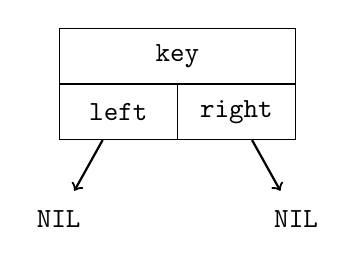
\begin{tikzpicture}
		[font=\ttfamily,minimum height=.7cm]
		\node (Key) [rectangle,draw,minimum width=3cm] {\texttt{key}};
		\node (LeftChild) [rectangle,draw,anchor=north west,minimum width=1.5cm] at (Key.south west) {\texttt{left}};
		\node (RightChild) [rectangle,draw,anchor=north east,minimum width=1.5cm] at (Key.south east) {\texttt{right}};
		\node[name=n1,yshift=-1cm] at (LeftChild.south west){NIL};
		\node[name=n2,yshift=-1cm] at (RightChild.south east){NIL};
		\draw[->, thick](RightChild) -- (n2);
		\draw[->,thick](LeftChild)--(n1);
	\end{tikzpicture}
\end{center}
Per risolvere tale problema, osserviamo che la prima sottochiamata viene effettuata sempre sul sottoalbero sinistro quindi, se ad un certo punto dell'iterazione si vede che \texttt{last} è uguale a \texttt{NIL} vorrà dire che la chiamata appena terminata è quella di sinistra. Si ha quindi:
\begin{lstlisting}[caption={\textsc{Search\_Iter}(T,k)},language=asd]
ct = T
start = true
stackT = NIL
while (start || stackT @$\neq$@ NIL) do
	ret = ct
	if (start) then
		if (ct @$\rightarrow$@ key @$\neq$@ k) then
			// Salvataggio contesto
			stackT = push(stackT, ct)
			ct = ct @$\rightarrow$@ left
		else
			result = ret
			start = false
			last = ct
		else
			// Ripristino contesto
			ct = top(stackT)
			// Individuazione punto di ritorno
			if (last = ct @$\rightarrow$@ left && ct @$\rightarrow$@ right @$\neq$@ NIL) then
				ret = result
				if (ret = NIL) then
					ct = ct @$\rightarrow$@ right
					start = true
				else
					stackT = pop(stackT)
					result = ret
					last = ct
			else
				stackT = pop(stackT)
				result = ret
				last = ct
return ret
\end{lstlisting}

\subsection{L'algoritmo PrintTree}
Consideriamo adesso l'algoritmo che si occupa di stampare in post-ordine le chiavi dei nodi presenti in un albero binario:
\begin{lstlisting}[language=asd,label=lst:print_tree,caption={\textsc{PrintTree}(T)}]
	if T@$\neq$@ NIL then
		PrintTree(T@$\rightarrow$@ left)
		PrintTree(T@$\rightarrow$@ right)
		print(T@$\rightarrow$@ key)
\end{lstlisting}
Dal momento che le varie sottochiamate vengono applicate su sottoalberi diversi sarà necessario salvare in uno stack il riferimento al sottoalbero corrente nel momento in cui si effettua una chiamata ricorsiva. Si ha quindi:
\begin{lstlisting}[language=asd,caption={\textsc{PrintTree\_Iter}(T)}]
ct = T
start = true
stackT = NIL
while (start || stackT @$\neq$@ NIL) do
	if (start) then
		if (ct @$\neq$@ NIL) then
			// Salvataggio contesto
			stackT = push(stackT, ct)
			ct = ct @$\rightarrow$@ left
		else
			last = ct
			start = false
	else
		ct = top(stackT)
		// Individuazione punto di ritorno
		if (last = ct @$\rightarrow$@ left && ct @$\rightarrow$@ right @$\neq$@ NIL) then
			ct = ct @$\rightarrow$@ right
			start = true
		// Fine della seconda sottochiamata
		else
			print(ct @$\rightarrow$@ key)
			stackT = pop(stackT)
			last = ct
\end{lstlisting}
\section{La ricorsione in coda}
Come detto all'inizio del capitolo la ricorsione può richiedere una grande allocazione di memoria dato dallo stack dei record di attivazione per ognuna delle chiamate effettuate col rischio di incorrere in overflow di memoria.

\begin{example}
	Si può dimostrare, ad esempio, che nell'esecuzione dell'Algoritmo \textsc{Fib}$(n)$ (Algoritmo \ref{lst:fibR}) le chiamate \textsc{Fib}$(0)$ e \textsc{Fib}$(1)$ sono calcolati \textsc{Fib}$(n+1)$ volte. Nella computazione di \textsc{Fib}$(29)$ sono chiamati $832040 = $ \textsc{Fib}$(30)$ volte.
	\begin{center}
		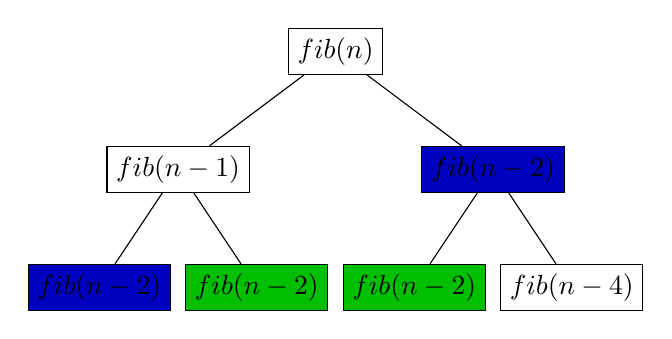
\begin{tikzpicture}
			[every node/.style={rectangle, draw},
			level 1/.style={sibling distance=4cm},
			level 2/.style={sibling distance =2cm}]
			\node{$fib(n)$}
			child
			{
				node{$fib(n-1)$}
				child
				{
					node[fill=blue!75!black]{$fib(n-2)$}
				}
				child
				{
					node[fill=green!75!black]{$fib(n-2)$}
				}
			}
			child
			{
				node[fill=blue!75!black]{$fib(n-2)$}
				child
				{
					node[fill=green!75!black]{$fib(n-2)$}
				}
				child
				{
					node{$fib(n-4)$}
				}
			};
		\end{tikzpicture}
	\end{center}
\end{example}
Per evitare tale dispendio di memoria è possibile pensare di costruire una ricorsione definita in modo tale che nel caso ricorsivo l'\textbf{ultima operazione} da eseguire è la chiamata ricorsiva. Infatti, se l'ultima istruzione effettuata nella funzione chiamante risulta la chiamata ricorsiva, allora non è necessario specificare alcun indirizzo di ritorno nella funzione chiamante ed è possibile sostituire tale valore con l'indirizzo di ritorno della funzione principale da cui la ricorsiva veniva chiamata.

Consideriamo ad esempio l'algoritmo di ricerca sugli alberi binari di ricerca:
\begin{lstlisting}[language=asd,caption={\textsc{SearchABR}(T,k)}]
ret = T
if T @$\neq$@ NIL then
	if (T@$\rightarrow$@ key < k) then
		ret = SearchABR(T @$\rightarrow$@ right, k)
	else if (T@$\rightarrow$@ key > k) then
		ret = SearchABR(T @$\rightarrow$@ left, k)
return ret
\end{lstlisting}
In questa situazione si osserva che non è assolutamente necessario salvare il contesto degli antenati (le chiamate padri) in quanto il calcolo della variabile \texttt{ret} avviene in modo indipendente dai suoi precedenti. Non è pertanto necessaria alcuna memoria aggiuntiva in quanto la ricerca di un nodo si riduce, nel caso degli alberi binari di ricerca, alla discesa lungo un percorso ben definito.

\begin{lstlisting}[language=asd,caption={\textsc{SearchABR\_Iter}(T,k)}]
ret = T
while (ret @$\neq$@ NIL && ret @$\rightarrow$@ key @$\neq$@ k) do
	if (ret @$\rightarrow$@ key < k) then
		ret = ret @$\rightarrow$@ right
	else
		ret = ret @$\rightarrow$@ left
return ret
\end{lstlisting}

La categoria di algoritmi per i quali non serve uno stack per il salvataggio del contesto adoperano una tipologia di ricorsione che prende il nome di \textbf{ricorsione in coda}. Sintatticamente, la ricorsione in coda corrisponde ad un algoritmo che effettua una sola chiamata ricorsiva senza dover effettuare infine una risalita\footnote{Per convenzione gli stack evolvono verso il basso.} lungo lo stack di attivazione per il recupero del contesto precedente. In modo del tutto analogo è possibile riscrivere l'algoritmo ricorsivo \ref{lst:factR} per il calcolo del fattoriale $n!$ in modo tale che effettui una ricorsione in coda:
\begin{lstlisting}[language=asd,caption={\textsc{Fattoriale\_Iter}(N)}]
t = 1
while (n>0) do
	t = t*n
	n = n-1
return t
\end{lstlisting}

Come si può osservare, non è necessario alcuno stack per il salvataggio del contesto delle chiamate interrotte in quanto il calcolo del risultato altro non fa che utilizzare le variabili condivise nel corso dell'iterazione: \texttt{t} per il calcolo del risultato e il parametro attuale \texttt{n} che viene decrementato di iterazione in iterazione.
